%!TEX root = /Users/simo/Documents/PFC/Chapter3/chapter3.tex
\section{Quinto Ciclo} % (fold)
\label{sec:quinto_ciclo}

En este ciclo se pretende tratar un tema que se ha dejado de banda desde el principio, que es la subida de archivos (pdf's o imágenes) para hacer de fondo en las páginas de los documentos. Debido a la naturaleza compleja de la tarea se ha preferido dejar para las últimas etapas del desarrollo, cuando hubiera una comprensión mayor del funcionamiento de Ruby on Rails.

\subsection{Análisis de requisitos} % (fold)
\label{sub:análisis_de_requisitos}

\begin{itemize}
  \item Poder crear páginas en blanco.
  \item Poder subir imágenes una a una creando páginas para el documento con ellas.
  \item Poder subir archivos comprimidos con imágenes dentro, que creen una página por cada imagen que se encuentre en el archivo. Las páginas se deberían ordenarán alfabéticamente según el nombre del archivo de la imagen. Como opción básica, se debe poder subir archivos zip, pero idealmente se debería poder subir otros formatos comunes, como rar o gz.
  \item Poder subir PDF's, que automáticamente convertirían cada página a una imagen, asignándola a una página nueva.
\end{itemize}

% subsection análisis_de_requisitos (end)

\subsection{Diseño} % (fold)
\label{sub:diseño}

\begin{figure}[h!]
\centering
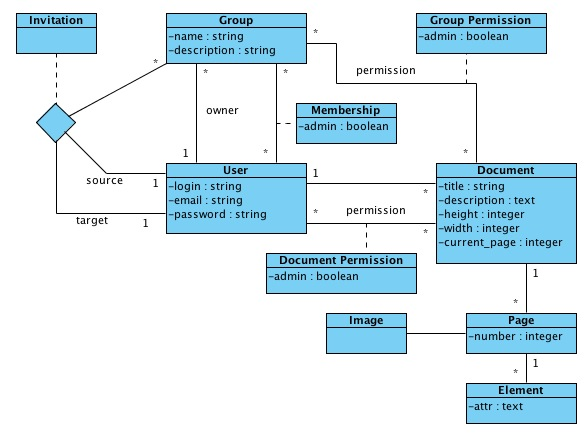
\includegraphics[width=14cm]{uml5.png}
\caption{Clases del dominio, 5º ciclo}\label{fig:uml5}
\end{figure}

Debido a lecturas en ciclos anteriores se conoce que el proceso de subir imágenes es otro aspecto muy común de las páginas web, y por lo tanto existe un Plugin excelente que da todas las herramientas necesarias para subir, generar thumbnails y almacenar imágenes en distintos soportes. Estos plugins generalmente requieren de un modelo extra que representará las imágenes, y que, como cualquier otro modelo dentro de Rails, se puede relacionar con el resto. Por tanto, aprovechando este conocimiento, se puede planear ya este modelo, y asignarlo, lógicamente, al modelo \texttt{Page}.

Este modelo solo tiene los atributos creados por el plugin, por lo cual se obvian en beneficio de una mayor claridad del diagrama.

% subsection diseño (end)

\subsection{Implementación} % (fold)
\label{sub:implementación}

La forma en que se plantearán estas funcionalidades, serán mostrando una columna lateral en la edición de un documento, separada del formulario de edición del documento y de administración de permisos, mediante el cual se mostrarían miniaturas de las páginas, y se podrían ir añadiendo páginas mediante las opciones disponibles. 

\subsubsection{Páginas en blanco} % (fold)
\label{ssub:paginas_en_blanco}

Esta es la opción más sencilla, y no necesita más que una acción que cree una página de la misma forma que se creaban anteriormente, cuando se generaba una cantidad de páginas fija. De la misma forma, es posible añadir una opción para generar un número de páginas, establecido por el usuario rellenando un campo de texto.

% subsubsection paginas_en_blanco (end)

\subsubsection{Subir imágenes una a una} % (fold)
\label{ssub:subir_imagenes_una_a_una}

Esta opción es el ejemplo clásico de uso de un plugin para subir archivos. El plugin utilizado en este caso es \texttt{attachment-fu} \footnote{http://github.com/technoweenie/attachment\_fu} , el cual, añadiendo unas líneas como las siguientes, hace que se relacione directamente con los archivos subidos mediante la interfaz web.

\begin{verbatim}
class Image < ActiveRecord::Base
  belongs_to :page
  
  has_attachment  :content_type => :image,
                  :processor => 'MiniMagick',
                  :thumbnails => {:small => '85x>',
                                  :medium => '360x360>',
                                  :big => '800x800>'},
                  :storage => :file_system,
                  :path_prefix => "/document_images/"
end
\end{verbatim}

Introduciendo esto en \texttt{/app/models/image.rb}, y al crear un objeto de tipo Image, pasándole como parámetro el input en el que se el usuario añade el archivo, hará las siguientes acciones:

\begin{itemize}
  \item Comprobará que es una imagen, porque se le ha pasado el parámetro \texttt{:content\_type => :image}. En caso de no ser un archivo de tipo imagen válido, fallará el momento de crear el objeto, es decir, al realizar un \texttt{save} o un \texttt{create} sobre \texttt{Image}.
  \item Generará tres thumbnails, con los tamaños especificados usando el formato clásico de \texttt{ImageMagick} \footnote{http://imagemagick.org/script/command-line-options.php\#resize}, mediante \texttt{MiniMagick} \footnote{http://rubyforge.org/projects/mini-magick/}.
  \item Guardará las imágenes en la carpeta \texttt{/document\_images}. Puesto que se le ha especificado claramente que está en la raíz de la aplicación, las guardará ahí, y no en \texttt{public}, que es lo normal. \texttt{public} es la carpeta que está abierta al público, y si se guardara en \texttt{/public/document\_images} en vez de en \texttt{/document\_images}, cualquier persona podría acceder a las imágenes mediante la dirección pública como \texttt{http://dominio.com/document\_images/..}
  
  De esta forma las imágenes están fuera del alcance, y se deberán servir mediante un método que lea este archivo y lo transmita, que al ser programado especialmente, puede controlar que el usuario que está reclamando una imagen tenga permisos para ver el documento, y no esté intentando ver documentos del resto.
\end{itemize}

Con la siguiente instrucción:

\begin{verbatim}
  render :file => image.public_filename(params[:thumb])
\end{verbatim}

es posible renderizar dicha imagen, de la misma forma que si accediera desde la dirección pública, pero estando dicha imagen fuera del alcance de todo el mundo, y pudiendo realizar las comprobaciones pertinentes.

% subsubsection subir_imagenes_una_a_una (end)

\subsubsection{Subiendo imágenes en un archivo comprimido} % (fold)
\label{ssub:subiendo_imágenes_en_un_archivo_comprimido}

Esta segunda opción añade una complicación básica, en que ninguno de los plugins existentes permiten hacer nada parecido a lo necesario aquí, por lo que debe hacerse todo a mano. La forma en que funcionan las subidas mediante web, en cualquier sistema, es que el servidor genera un archivo temporal conteniendo el archivo en si, y que Ruby on Rails permite acceder de forma normal, igual que se accede a cualquiera de los parámetros rellenados en un formulario, pero en vez de ser un \texttt{String}, es un \texttt{Tempfile} \footnote{\url{http://corelib.rubyonrails.org/classes/Tempfile.html}}. 

Puesto que es un archivo que se deberá descomprimir, y después realizar las acciones necesarias para generar páginas con las imágenes descomprimidas, es necesario algún tipo de organización de directorios para poder trabajar de forma temporal, y sin que pueda haber interferencias entre varios procesos descomprimiendo al mismo tiempo. La carpeta \texttt{/document\_temp} contendrá una serie de carpetas que se irán creando cuyo nombre será el timestamp del momento de la subida, concatenado con el identificador del documento para el cual se están subiendo imágenes. De esta forma, se puede en un futuro tener un control de carpetas que quizá hayan quedado descontroladas por algún proceso interrumpido de forma inesperada, siempre controlado que por ejemplo, dichas carpetas temporales hayan sido creadas hace más de una hora.

Dicha previsión se cree conveniente para poder blindar el proceso, y que ningún posible error en el código, o subidas de archivos maliciosos puedan ocupar espacio indeseado.

Mediante Ruby, igual que con cualquier otro lenguaje, es posible realizar todo tipo de operaciones de movimiento de archivos y creación de carpetas, por lo que crear dicha carpeta y eliminarla al final no es problema. El siguiente reto es conseguir descomprimir un archivo, en principio, desconocido, y por supuesto, contra más flexibilidad mejor. Existe un descompresor llamado \texttt{e}, de Martin Ankerl \footnote{\url{http://martin.ankerl.com/2006/08/11/program-e-extract-any-archive/}}, que al estar escrito en Ruby, es muy fácilmente adaptable a las necesidades de este proyecto. El código utilizado por este descompresor soporta hasta un límite de 32 formatos distintos, siempre y cuando esté el descompresor necesario instalado en el sistema.

Una vez descomprimidas las imágenes, existe el problema de la organización interna del fichero. ¿Qué pasa si existen varias carpetas? En este punto se corre el riesgo de complicar extremadamente la cosa, puesto que no siempre se puede saber cuál es la intención del usuario a la hora de subir las imágenes comprimidas en varias carpetas. En este caso, se ha tomado la política de extraer todas las imágenes, independientemente de la carpeta en que estén, y añadirlas de forma ordenada alfabéticamente.

Para hacer esto, de nuevo, aparentemente complejo, no hay más que usar uno de los módulos de la librería básica de Ruby, \texttt{Find} \footnote{\url{http://corelib.rubyonrails.org/classes/Find.html}}, el cual permite recorrer recursivamente una estructura de directorios, a partir de la cual generar un vector de archivos, referenciables posteriormente. Mediante este vector, y la función \texttt{File.basename}, es posible ordenar los archivos, guardados en el vector \texttt{files}, con la siguiente línea:

\begin{verbatim}
  files.sort! {|a,b| File.basename(a) <=> File.basename(b)}
\end{verbatim}

Ruby, de nuevo, ya tiene un algoritmo de ordenación implementado, al cual se le puede explicar por qué parámetro ordenar un vector, en este caso, por los nombres de archivo.

Teniendo, pues, un vector con referencias a las imágenes, ya comprimidas y ordenadas alfabéticamente solo queda generar las páginas con sus elementos \texttt{Image} generados. Mediante otra línea de texto explicada en la documentación del plugin \texttt{attachment-fu}, es fácilmente generable objetos de este tipo a partir de archivos ya existentes en el servidor.

% subsubsection subiendo_imágenes_en_un_archivo_comprimido (end)

\subsubsection{Subiendo archivos PDF} % (fold)
\label{ssub:subiendo_archivos_pdf}

Éste, a pesar de lo que pueda parecer, es un problema muy semejante al proceso anterior. El proceso de convertir de un archivo PDF a imágenes es posible gracias a la herramienta \texttt{ImageMagick}, un standard de facto en cualquier servidor web para el proceso de imágenes, que se ha usado tradicionalmente para la generación de thumbnails, redimensionado de imágenes, ademas de otras tareas un tanto más avanzadas como la adición de marcas de agua a imágenes. Entre sus posibilidades, existe la posibilidad de convertir entre cualquiera de los formatos soportados, encontrándose PDF entre ellos. Convertir de un PDF a una serie de imágenes es posible mediante el comando:

\begin{verbatim}
  $ convert file.pdf image.jpg
\end{verbatim}

Generando una imagen por página con los nombres \texttt{image0.jpg}, \texttt{image1.jpg}, etc. Teniendo, pues, estas imágenes descomprimidas en un directorio, no hay más que seguir el mismo proceso que con las imágenes descomprimidas para crear las páginas necesarias.

% subsubsection subiendo_archivos_pdf (end)

\subsubsection{Otras posibilidades} % (fold)
\label{ssub:otras_posibilidades}

Una de las posibilidades que se barajó el etapas preliminares del proyecto, fue la posibilidad de subir presentaciones PowerPoint directamente, puesto que es uno de los formatos más usados para presentaciones, y al fin y al cabo el objetivo básico de esta aplicación es facilitar dichas presentaciones cuando deben realizarse a distancia.

Esta tarea, sin embargo, es prácticamente imposible presuponiendo que la aplicación funcionará sobre una plataforma Unix, lo más normal en cualquier servidor web. En caso de estar funcionando en una plataforma Windows, sería posible mediante los componentes OLE32. En cualquier otro caso, este problema no se ha podido resolver.

% subsubsection otras_posibilidades (end)

% subsection implementación (end)

% section cuarto_ciclo (end)